\documentclass[11pt,a4paper]{article}

% ── Packages ────────────────────────────────────────────────────────────────
\usepackage[T1]{fontenc}
\usepackage[utf8]{inputenc}
\IfFileExists{lmodern.sty}{\usepackage{lmodern}}{}
% Use lmodern if available; otherwise disable microtype font expansion,
% which requires a scalable font (Type1) to be present.
\IfFileExists{lmodern.sty}{\usepackage{microtype}}{\usepackage[expansion=false]{microtype}}
\usepackage[a4paper, top=2.5cm, bottom=2.5cm, left=2.3cm, right=2.3cm]{geometry}
\usepackage{amsmath,amssymb,amsthm}
\usepackage{graphicx}
\usepackage{booktabs}
\usepackage{array}
\usepackage{hyperref}
\usepackage{xcolor}
\usepackage{listings}
\usepackage{caption}
\usepackage{subcaption}
\usepackage{enumitem}
\usepackage{fancyhdr}
\usepackage{titlesec}
\usepackage[numbers,compress]{natbib}
\usepackage{multicol}
\usepackage{float}

% ── Hyperref ────────────────────────────────────────────────────────────────
\hypersetup{colorlinks=true,linkcolor=blue!60!black,
            citecolor=green!40!black,urlcolor=blue!70!black}

% ── Code style ──────────────────────────────────────────────────────────────
\lstset{
  language=Python, basicstyle=\ttfamily\footnotesize,
  keywordstyle=\color{blue!70!black}\bfseries,
  commentstyle=\color{gray}\itshape,
  showstringspaces=false, breaklines=true,
  frame=single, rulecolor=\color{gray!30},
  backgroundcolor=\color{gray!4},
  numbers=none, xleftmargin=6pt, xrightmargin=6pt,
  aboveskip=4pt, belowskip=4pt,
}

% ── Section formatting ───────────────────────────────────────────────────────
\titleformat{\section}{\large\bfseries}{\thesection.}{0.5em}{}[\titlerule]
\titleformat{\subsection}{\normalsize\bfseries}{\thesubsection}{0.5em}{}
\titlespacing{\section}{0pt}{10pt}{5pt}
\titlespacing{\subsection}{0pt}{7pt}{3pt}

% ── Header / footer ─────────────────────────────────────────────────────────
\pagestyle{fancy}\fancyhf{}
\lhead{\small\textit{Assignment 5 — Clustering and Initialization}}
\rhead{\small Statistical Methods for Machine Learning, A.Y.\ 2025/26}
\rfoot{\small\thepage}
\renewcommand{\headrulewidth}{0.4pt}

% ── Theorem environments ─────────────────────────────────────────────────────
\newtheorem{theorem}{Theorem}

% ── Macros ───────────────────────────────────────────────────────────────────
\newcommand{\kpp}{$k$\text{-means++}}
\newcommand{\km}{$k$\text{-means}}
\newcommand{\Rbb}{\mathbb{R}}
\newcommand{\EE}{\mathbb{E}}
\newcommand{\norm}[1]{\lVert #1 \rVert}
\setlength{\parskip}{4pt}
\setlength{\parindent}{0pt}
\captionsetup{font=small,labelfont=bf,skip=6pt}

% ════════════════════════════════════════════════════════════════════════════
\begin{document}
% ════════════════════════════════════════════════════════════════════════════

% ── Compact title block ─────────────────────────────────────────────────────
\begin{center}
  {\LARGE\bfseries Assignment 5 — Clustering and Initialization}\\[4pt]
  {\large\itshape $k$-means vs $k$-means++: The Advantages of Careful Seeding}\\[8pt]
  {\small Statistical Methods for Machine Learning $\cdot$
   Università degli Studi di Milano $\cdot$
   Instructor: Nicolò Cesa-Bianchi}\\[4pt]
  {\small\textbf{Student:} Srishti Kansra \quad \textbf{ID:} 49483A }
\end{center}

\smallskip
\noindent\fbox{\parbox{\dimexpr\linewidth-2\fboxsep-2\fboxrule\relax}{%
  \footnotesize\itshape
  I declare that this material, which I now submit for assessment, is entirely my own work and has not been taken from the work of others, save and to the extent that such work has been cited and acknowledged within the text of my work. I understand that plagiarism, collusion, and copying are grave and serious offences in the university and accept the penalties that would be imposed should I engage in plagiarism, collusion or copying. This assignment, or any part of it, has not been previously submitted by me or any other person for assessment on this or any other course of study.}}
\vspace{4pt}

% ════════════════════════════════════════════════════════════════════════════
\section{Introduction}
% ════════════════════════════════════════════════════════════════════════════

Given $n$ data points $x_1,\ldots,x_n\!\in\!\Rbb^d$ and a target cluster count $k$,
$k$-means seeks centers $c_1,\ldots,c_k$ minimizing the \emph{inertia}:
\begin{equation}
  \phi = \sum_{i=1}^{n}\min_{j}\norm{x_i-c_j}^2. \label{eq:inertia}
\end{equation}
Because $\phi$ is non-convex, Lloyd's algorithm [2] only converges to a
\emph{local} minimum; which minimum depends entirely on the initial centers.
This project compares two initialization strategies under controlled conditions:
\textbf{random (Forgy)} — $k$ centers drawn uniformly at random — and
\textbf{$k$-means++} [1] — centers seeded sequentially with
probability proportional to the squared distance to the nearest existing center ($D^2$
weighting). The methods are identical in every other respect.

Evaluation covers four axes across three datasets: \textbf{inertia} (internal),
\textbf{ARI} and \textbf{NMI} (external, against ground-truth labels),
\textbf{convergence speed} (Lloyd iterations), and \textbf{run-to-run stability}.
All algorithms and metrics are implemented from scratch in NumPy;
\texttt{scikit-learn} is used only to generate or load raw data.

% ════════════════════════════════════════════════════════════════════════════
\section{Datasets and Pre-processing}
% ════════════════════════════════════════════════════════════════════════════

\begin{table}[H]
\centering\small
\caption{Datasets used. The assignment requires at least one synthetic and one real-world
         dataset; overlapping clusters and the $k$-sweep set are extensions.}
\label{tab:datasets}
\begin{tabular}{llccl}
\toprule
\textbf{Dataset} & \textbf{Type} & $n\times d$ & $k$ & \textbf{Role} \\
\midrule
Well-separated clusters & Synthetic (\texttt{std=0.6}) & $500\times2$ & 5
  & Clean regime; ideal for $k$-means++ \\
Overlapping clusters & Synthetic (\texttt{std=1.8}) & $500\times2$ & 5
  & Weak-structure extension \\
Digits & Real-world, 10 digit classes & $1797\times64$ & 10
  & Required high-dimensional dataset \\
Varying-$k$ clusters & Synthetic (\texttt{std=0.5}, 15 true clusters)
  & $1000\times2$ & $2$--$15$ & Theory verification \\
\bottomrule
\end{tabular}
\end{table}

\textbf{Pre-processing choices.}
The synthetic cluster datasets require no preprocessing: \texttt{make\_blobs} generates
isotropic Gaussian clusters that are already well-scaled. The Digits dataset is
standardized to zero mean and unit variance per feature before clustering, because
$k$-means is not scale-invariant — features with larger absolute values dominate the
Euclidean distance and therefore the objective. Features with zero variance are set to
unit standard deviation to avoid division by zero.

\textbf{Reproducibility.} All experiments use \texttt{random\_state=42}, 50 independent
restarts, \texttt{max\_iter=300}, and \texttt{tol=}$10^{-4}$ (max center shift).
A critical implementation detail: the empty-cluster fallback draws from the same
\emph{seeded} generator as the rest of the run — not NumPy's global RNG — so every
step of a given \texttt{random\_state} is fully reproducible.

% ════════════════════════════════════════════════════════════════════════════
\section{Algorithms and Implementation}
% ════════════════════════════════════════════════════════════════════════════

\subsection{Theoretical background}

Lloyd's algorithm alternates (i) \textbf{assignment}: $\ell(x_i)=\arg\min_j\norm{x_i-c_j}^2$,
and (ii) \textbf{update}: $c_j\leftarrow|C_j|^{-1}\!\sum_{x\in C_j}\!x$. Each step
decreases $\phi$, guaranteeing convergence to a local minimum.

\textbf{$k$-means++ seeding.} Pick $c_1$ uniformly; then for each subsequent center
sample $x$ with $p(x)\propto D(x)^2=\min_{j<\ell}\norm{x-c_j}^2$. This $D^2$ weighting
spreads seeds away from existing centers at cost $O(knd)$, negligible versus Lloyd's
$O(I \cdot n \cdot k \cdot d)$ total cost. Its key guarantee is:
\begin{theorem}[Arthur \& Vassilvitskii, 2007~{\normalfont[1]}]
  $\EE[\phi_0]\leq 8(\ln k+2)\cdot\phi^*$,
  where $\phi^*$ is the optimal inertia and $\phi_0$ is the initialization cost.
\end{theorem}
This \emph{O$(\log k)$-competitive} bound concerns the quality of the seeding relative
to the optimum $\phi^*$; the approximation factor it guarantees loosens as $k$ grows.
It does not directly predict the empirical gap over random initialization, but it
motivates a related expectation we test in Section~\ref{sec:exp3}: with more clusters,
random init has more opportunities to seed two centers in one true cluster, so the gap
between the two methods should tend to widen with $k$.

\subsection{From-scratch implementation}

All code is NumPy-only. The central function is:
\begin{lstlisting}
def kmeans(X, k, init='random', random_state=None, max_iter=300, tol=1e-4):
    """Returns: centers (k,d), labels (n,), inertia (float), n_iter (int)."""
    rng     = np.random.default_rng(random_state)     # one seeded generator per run
    centers = INITIALIZERS[init](X, k, rng)           # pluggable init strategy
    for i in range(1, max_iter + 1):
        labels      = assign_labels(X, centers)        # vectorised: (n,k,d)->argmin
        new_centers = update_centers(X, labels, k, rng)
        if np.max(np.linalg.norm(new_centers - centers, axis=1)) < tol:
            break
        centers = new_centers
    labels  = assign_labels(X, centers)               # final labels from final centers
    return centers, labels, compute_inertia(X, labels, centers), i
\end{lstlisting}

The \texttt{INITIALIZERS} registry maps \texttt{'random'} to Forgy sampling and
\texttt{'kmeans++'} to the $D^2$ seeding loop; adding a new strategy requires only
inserting it into the registry. Assignment uses vectorized broadcasting
$(n,d)\to(n,k,d)\to\text{argmin}_{(n,)}$; the update step re-seeds empty clusters
from the seeded generator rather than the global RNG.

% ════════════════════════════════════════════════════════════════════════════
\section{Evaluation Metrics}
% ════════════════════════════════════════════════════════════════════════════

\textbf{Inertia} ($\phi$, Eq.~\ref{eq:inertia}) is the $k$-means objective — lower is
tighter — but it is not comparable across datasets (it scales with $n$, $d$, and feature
spread) and is decoupled from true cluster quality in high dimensions.
Because every dataset here has ground-truth labels we add two external metrics, both
implemented from scratch via a contingency table.

\textbf{Adjusted Rand Index (ARI)} [3] counts concordant pairs
and corrects for chance; ARI$=1$ for a perfect partition, ARI$\approx0$ for random
agreement. \textbf{Normalized Mutual Information (NMI)} measures shared information
between the predicted and true labelings, normalized by their mean entropy; NMI$=1$ is
perfect.

\textbf{Near-optimal fraction} $f_\tau = T^{-1}\sum_t\mathbf{1}[J_t\leq J^*(1+\tau)]$
(we use $\tau=0.01$) directly measures how often a method finds a near-optimal
solution across restarts, making it more interpretable than the coefficient of variation
(CV$=$std/mean).

\textbf{Paired seeds.} Both strategies are evaluated on the \emph{same} 50-seed
sequence, so any difference in outcomes is attributable to the initialization, not
to luck in the restart draw.

% ════════════════════════════════════════════════════════════════════════════
\section{Experiments and Results}
% ════════════════════════════════════════════════════════════════════════════

\subsection{Experiment 1: Well-separated clusters}
\label{sec:exp1}

\begin{table}[H]
\centering\small
\caption{Experiment 1 — well-separated clusters ($k=5$, 50 restarts).}
\label{tab:exp1}
\begin{tabular}{lrrrrrr}
\toprule
\textbf{Method} & \textbf{Mean $J$} & \textbf{Std $J$} & \textbf{CV}
  & \textbf{Near-opt} & \textbf{ARI} & \textbf{Iters} \\
\midrule
Random & 1109.2 & 889.6 & 80.2\% & 42\% & 0.833 & 5.58 \\
$k$-means++ & 439.4 & 331.8 & 75.5\% & 88\% & 0.966 & 3.10 \\
\bottomrule
\end{tabular}
\end{table}

\begin{figure}[H]
  \centering
  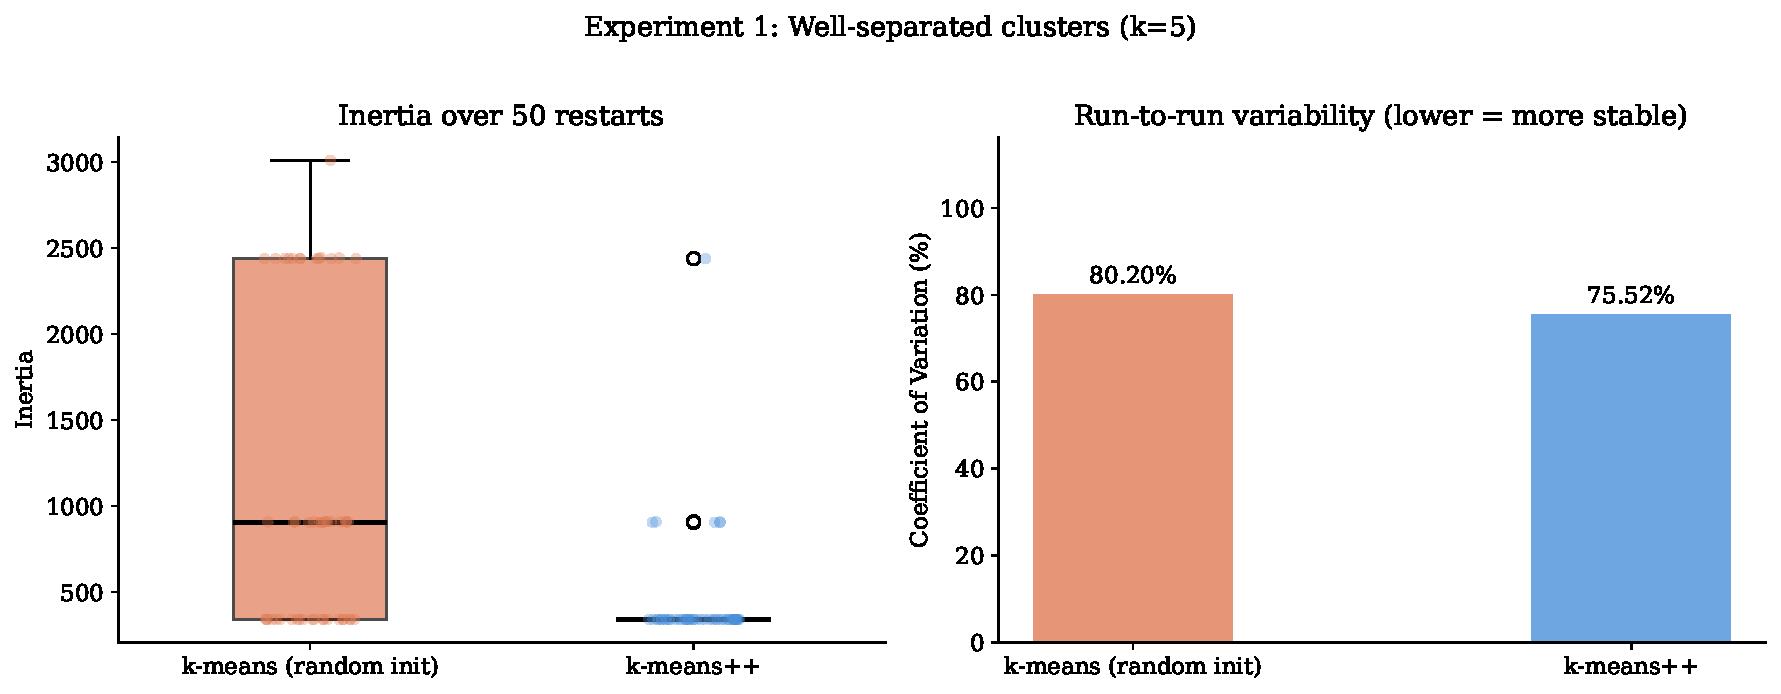
\includegraphics[width=\linewidth]{figures/exp1_separated.pdf}
  \caption{Inertia distribution and CV over 50 restarts — well-separated clusters.
           $k$-means++ is both lower and more consistent.}
  \label{fig:exp1_inertia}
\end{figure}

$k$-means++ outperforms random initialization on every axis. It reduces mean inertia by \textbf{60.4\%}
(439 vs 1109), raises ARI from 0.833 to \textbf{0.966} and NMI from 0.919 to 0.984,
and converges in \textbf{3.1 iterations} vs 5.6 — roughly half as many Lloyd steps.
The near-optimal fraction rises from 42\% to \textbf{88\%}: random init reaches a
near-optimal solution in fewer than half of its runs.

\begin{figure}[H]
  \centering
  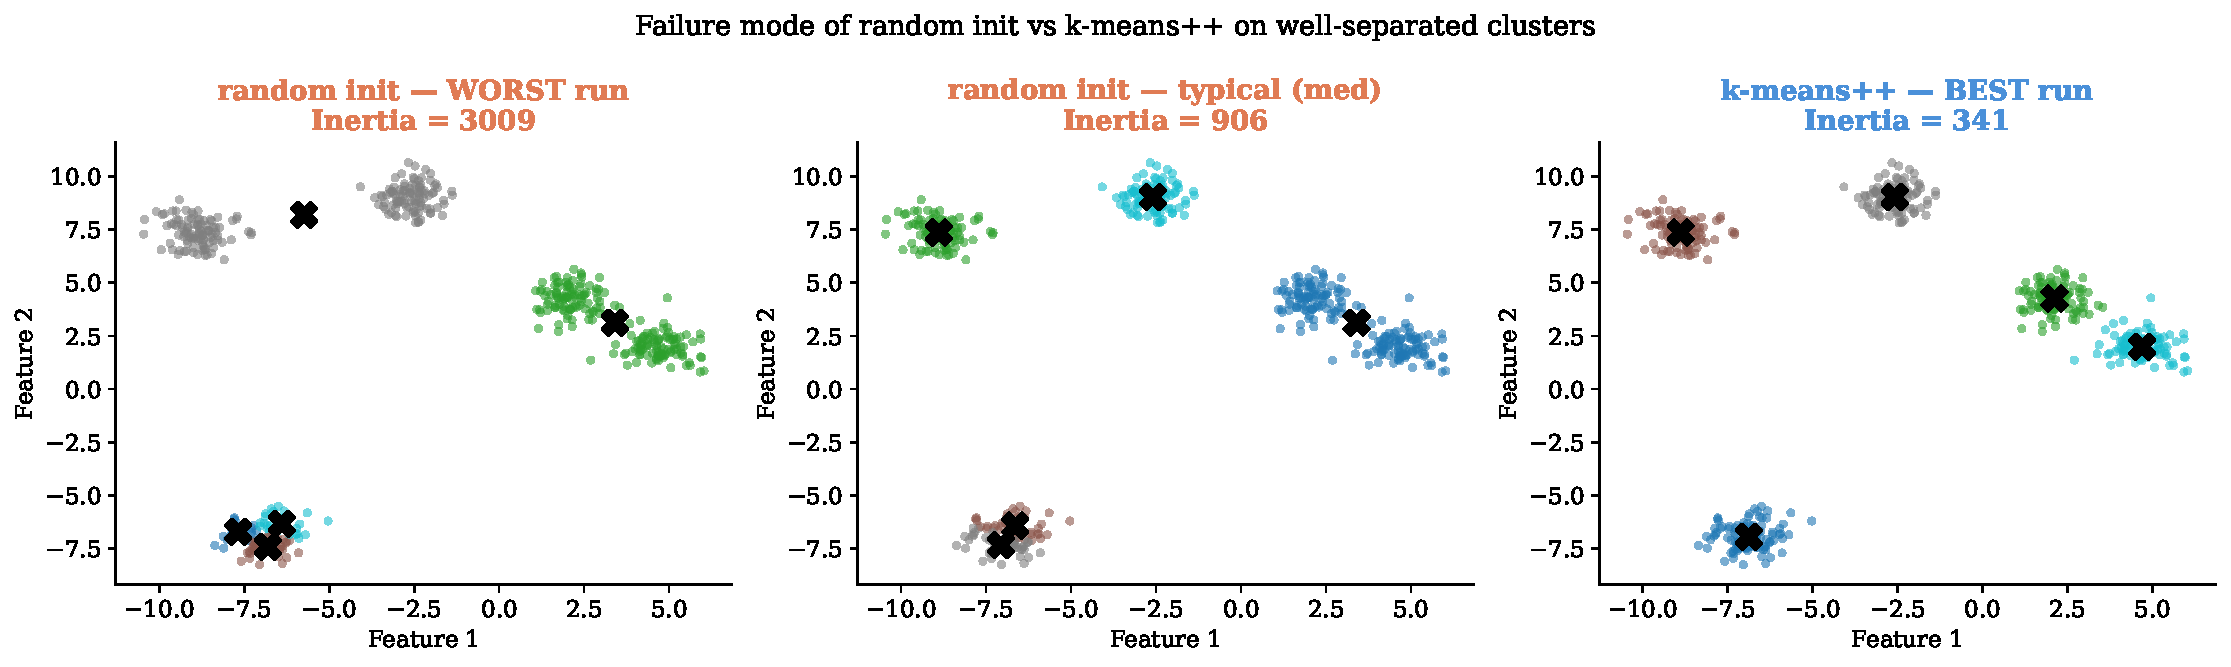
\includegraphics[width=\linewidth]{figures/exp1_scatter.pdf}
  \caption{Failure mode of random init. Left: the worst random run — two seeds in the
           same true cluster, locking in a bad local minimum. Center: a typical random
           run. Right: the best $k$-means++ run. Black crosses = final centers.}
  \label{fig:exp1_scatter}
\end{figure}

Figure~\ref{fig:exp1_scatter} shows the failure mechanism directly. In the worst random
run two seeds landed in the same cluster, splitting it while merging two adjacent ones.
Lloyd's updates often cannot recover from this — once centers are placed, every assignment step is
optimal \emph{given} those centers, and in this configuration no single reassignment splits the
merged cluster, so the run stays trapped in the sub-optimal partition. $k$-means++
avoids this by placing one seed in each cluster via the $D^2$ rule.

\begin{figure}[H]
  \centering
  \begin{subfigure}[b]{0.48\linewidth}
    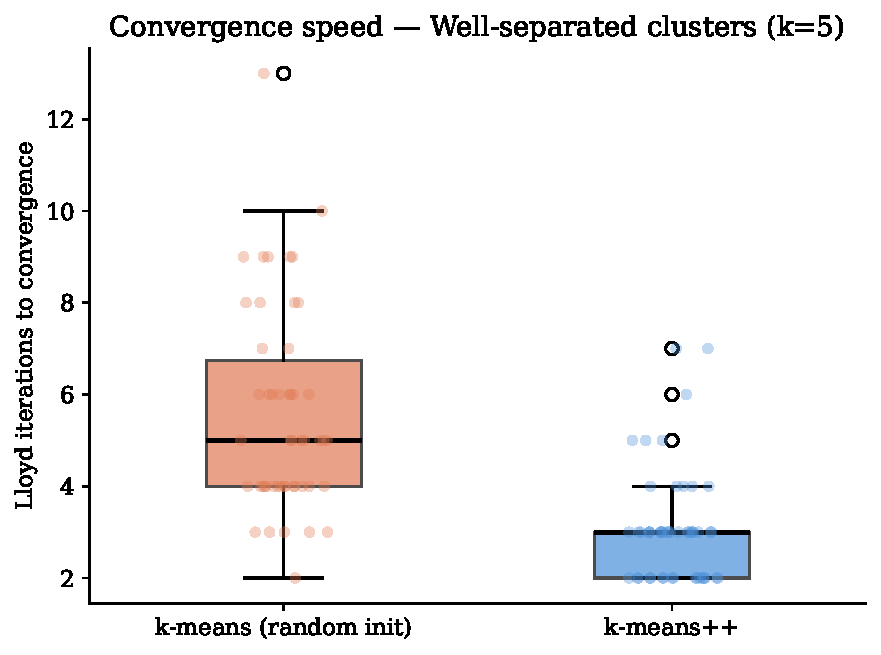
\includegraphics[width=\linewidth]{figures/exp1_iters.pdf}
    \caption{Convergence speed (iterations).}
    \label{fig:exp1_iters}
  \end{subfigure}\hfill
  \begin{subfigure}[b]{0.48\linewidth}
    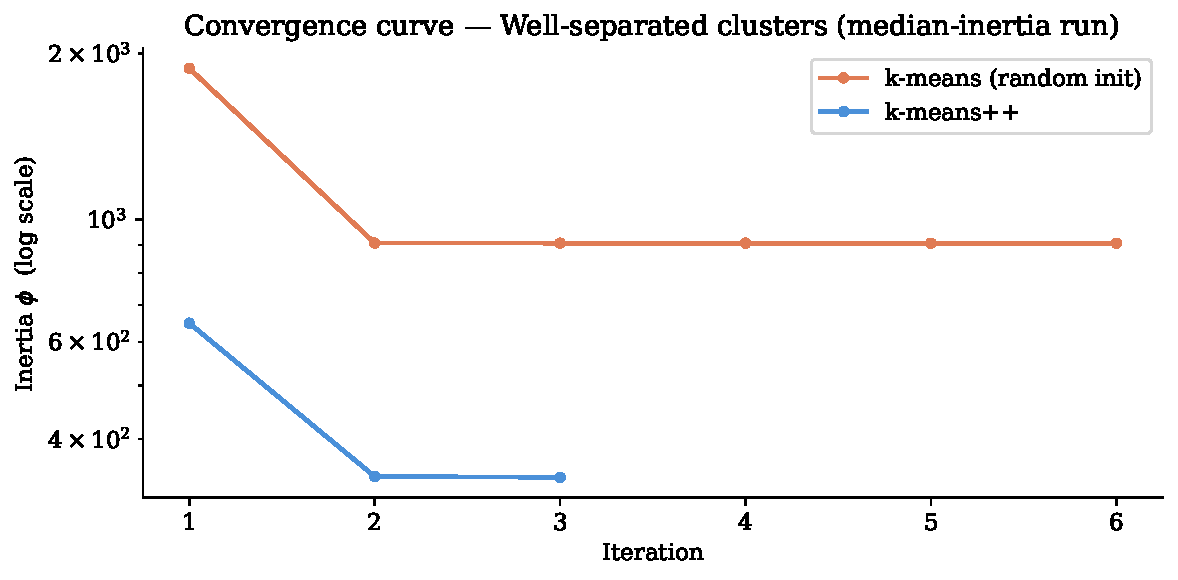
\includegraphics[width=\linewidth]{figures/exp1_convergence.pdf}
    \caption{Per-iteration inertia $\phi$ (median run).}
    \label{fig:exp1_conv}
  \end{subfigure}
  \caption{Left: $k$-means++ needs $\sim$half the Lloyd iterations.
           Right: inertia $\phi$ decreases monotonically across Lloyd iterations;
           $k$-means++ starts from a lower $\phi$ at iteration~1 (seeding advantage) and converges sooner.
           Convergence is guaranteed because Lloyd monotonically decreases $\phi$.}
  \label{fig:exp1_speed}
\end{figure}

\subsection{Experiment 2: Overlapping clusters}
\label{sec:exp2}

\begin{table}[H]
\centering\small
\caption{Experiment 2 — overlapping clusters ($k=5$, 50 restarts).}
\label{tab:exp2}
\begin{tabular}{lrrrrrr}
\toprule
\textbf{Method} & \textbf{Mean $J$} & \textbf{Std $J$} & \textbf{CV}
  & \textbf{Near-opt} & \textbf{ARI} & \textbf{Iters} \\
\midrule
Random & 2915.3 & 423.3 & 14.5\% & 74\% & 0.780 & 11.26 \\
$k$-means++ & 2930.8 & 273.6 & 9.3\% & 64\% & 0.768 & 9.42 \\
\bottomrule
\end{tabular}
\end{table}

\begin{figure}[H]
  \centering
  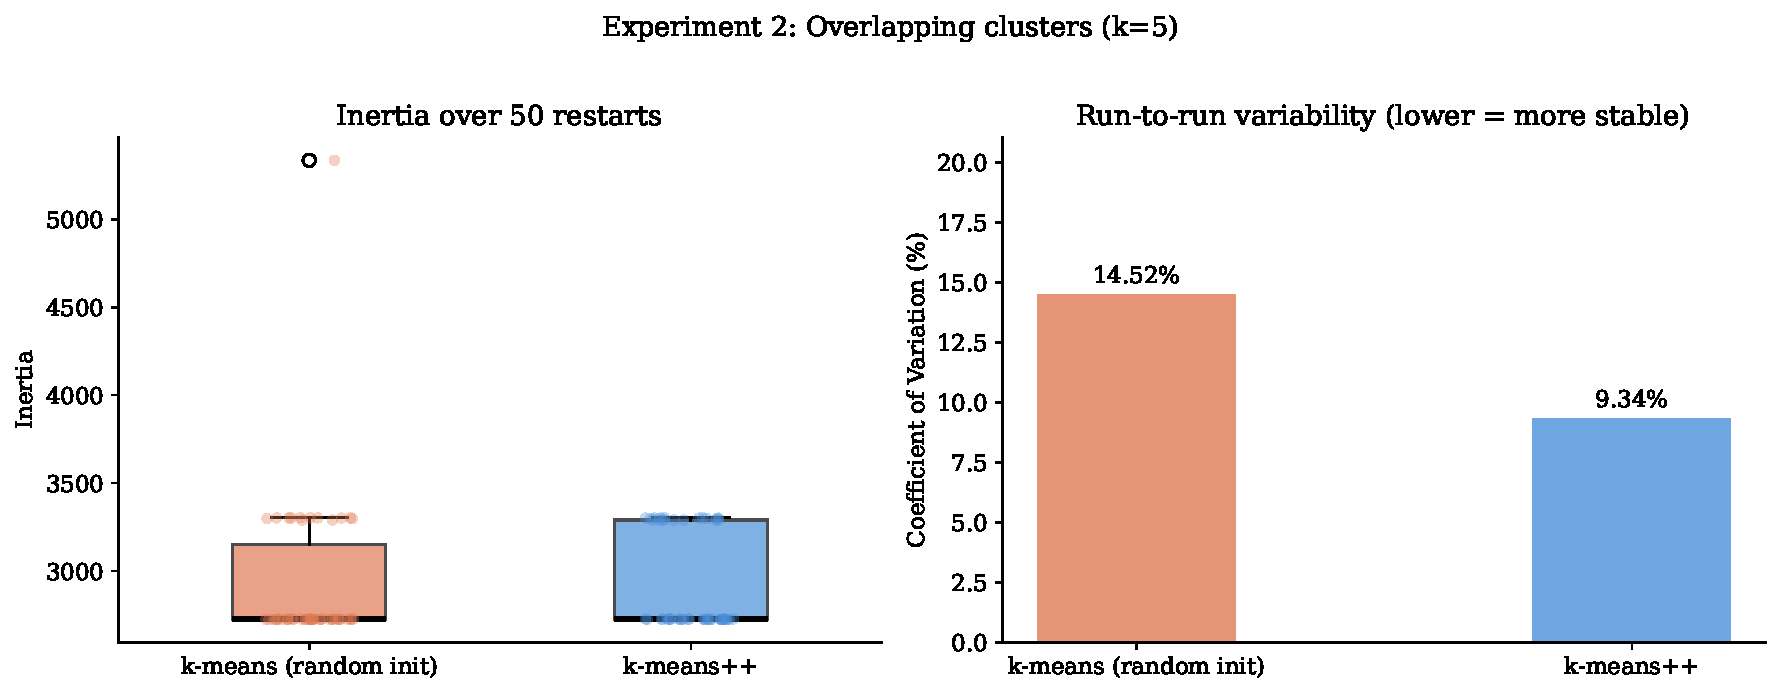
\includegraphics[width=\linewidth]{figures/exp2_overlapping.pdf}
  \caption{Overlapping clusters: similar mean inertia ($<0.5\%$ difference),
           but $k$-means++ has noticeably lower variability (CV 9.3\% vs 14.5\%).}
  \label{fig:exp2}
\end{figure}

The picture changes entirely. Both methods reach nearly identical inertia ($<0.5\%$
difference), and external quality is indistinguishable (ARI 0.780 vs 0.768, NMI 0.832
vs 0.828). $k$-means++ gains are now confined to \textbf{stability} (CV 9.3\% vs
14.5\%, a 36\% reduction) and \textbf{speed} (9.4 vs 11.3 iterations). When clusters
overlap substantially the objective landscape flattens — many configurations achieve
similar inertia — so the starting point is less consequential for final quality. The
near-optimal fraction even inverts (64\% vs 74\%): with a flat landscape the 1\%
tolerance threshold is easy to exceed, reflecting landscape ambiguity rather than
inferior performance.

\subsection{Experiment 3: Effect of $k$ and link to theory}
\label{sec:exp3}

\begin{figure}[H]
  \centering
  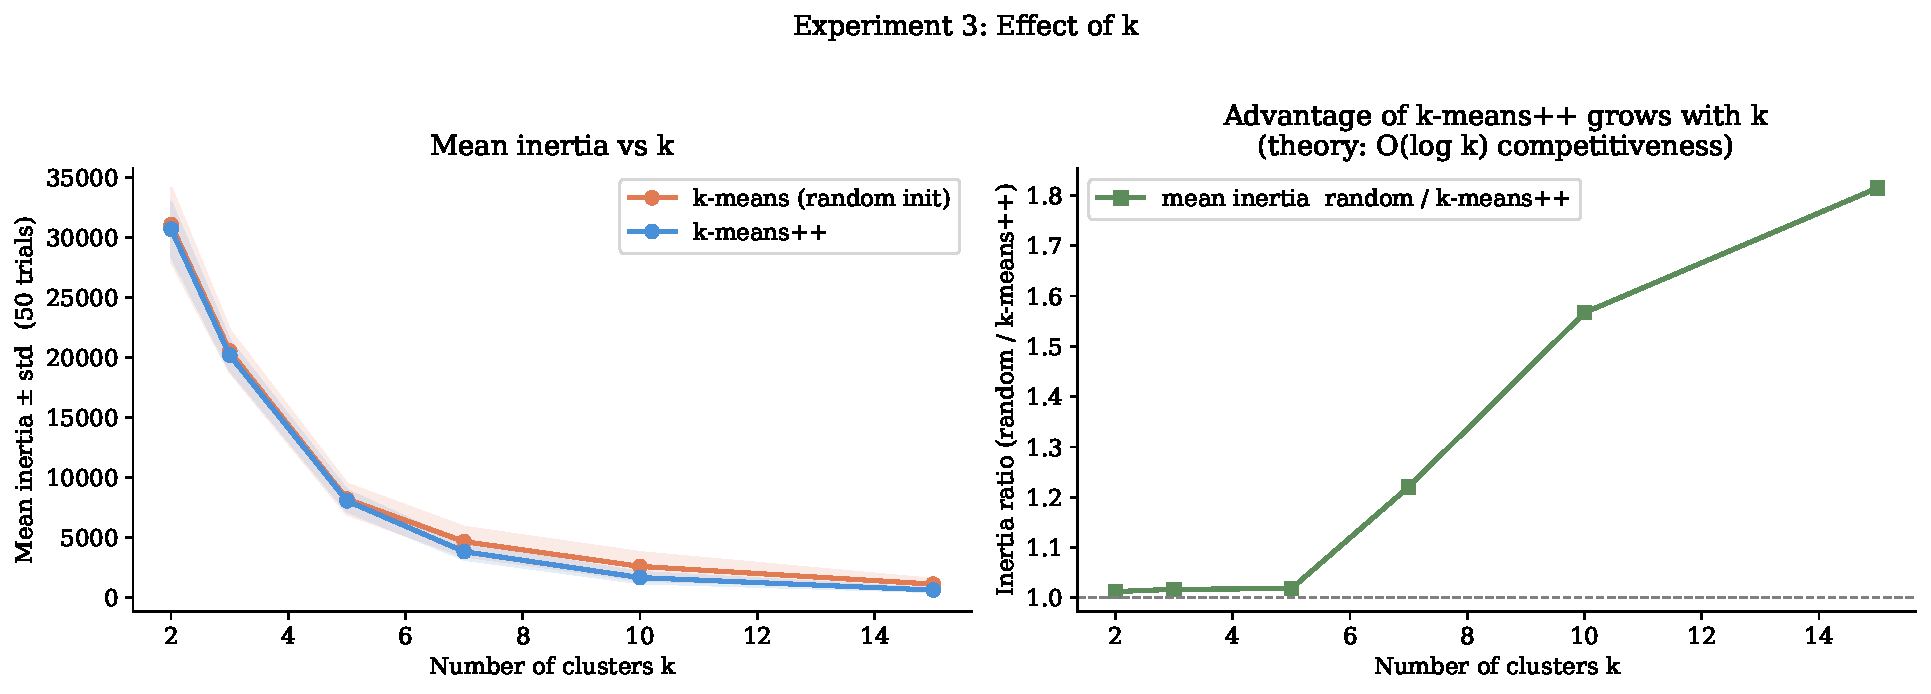
\includegraphics[width=\linewidth]{figures/exp3_vs_k.pdf}
  \caption{Left: mean inertia vs $k$. Right: random/$k$-means++ inertia ratio vs $k$.
           The ratio grows monotonically from 1.01 at $k=2$ to 1.82 at $k=15$,
           qualitatively consistent with the O$(\log k)$ guarantee that random init has
           more chances to mis-seed as $k$ grows.}
  \label{fig:exp3}
\end{figure}

\begin{table}[H]
\centering\small
\caption{Inertia ratio vs $k$: $\bar{J}_\text{rand}/\bar{J}_{++}$ increases with $k$.
The $\ln k$ column is shown for reference only; the ratio is a distinct quantity from
the theoretical $\ln k$ factor and is not expected to match it numerically.}
\label{tab:exp3}
\begin{tabular}{ccccc}
\toprule
$k$ & $\bar{J}_\text{rand}$ & $\bar{J}_{++}$ & \textbf{Ratio} & $\ln k$ \\
\midrule
2  & 31053 & 30675 & 1.012 & 0.69 \\
3  & 20519 & 20178 & 1.017 & 1.10 \\
5  &  8187 &  8041 & 1.018 & 1.61 \\
7  &  4643 &  3805 & 1.220 & 1.95 \\
10 &  2578 &  1645 & 1.567 & 2.30 \\
15 &  1099 &    606 & \textbf{1.815} & 2.71 \\
\bottomrule
\end{tabular}
\end{table}

The advantage of $k$-means++ grows \textbf{monotonically} from 1.012 at $k=2$ to
\textbf{1.815} at $k=15$ (Table~\ref{tab:exp3}). For small $k$ (2--5) the advantage is
negligible: with few clusters, random init rarely seeds two centers in the same cluster.
At $k=7$ the ratio jumps to 1.22 as seeding errors become frequent. The trend is
qualitatively consistent with the O$(\log k)$ competitive bound — more clusters give
random init more opportunities to mis-seed, widening the gap — though the inter-method
ratio is a different quantity from the bound's $\ln k$ factor and we make no claim that
the two match numerically.

\subsection{Experiment 4: Real-world high-dimensional data (Digits)}
\label{sec:exp4}

\begin{table}[H]
\centering\small
\caption{Experiment 4 — Digits ($d=64$, $k=10$, 50 restarts).}
\label{tab:exp4}
\begin{tabular}{lrrrrrr}
\toprule
\textbf{Method} & \textbf{Mean $J$} & \textbf{Std $J$} & \textbf{CV}
  & \textbf{Near-opt} & \textbf{ARI} & \textbf{Iters} \\
\midrule
Random      & 70{,}493 & 883 & 1.25\% & 42\% & \textbf{0.512} & 25.58 \\
$k$-means++ & 71{,}381 & 959 & 1.34\% & 16\% & 0.464          & 25.12 \\
\bottomrule
\end{tabular}
\end{table}

\begin{figure}[H]
  \centering
  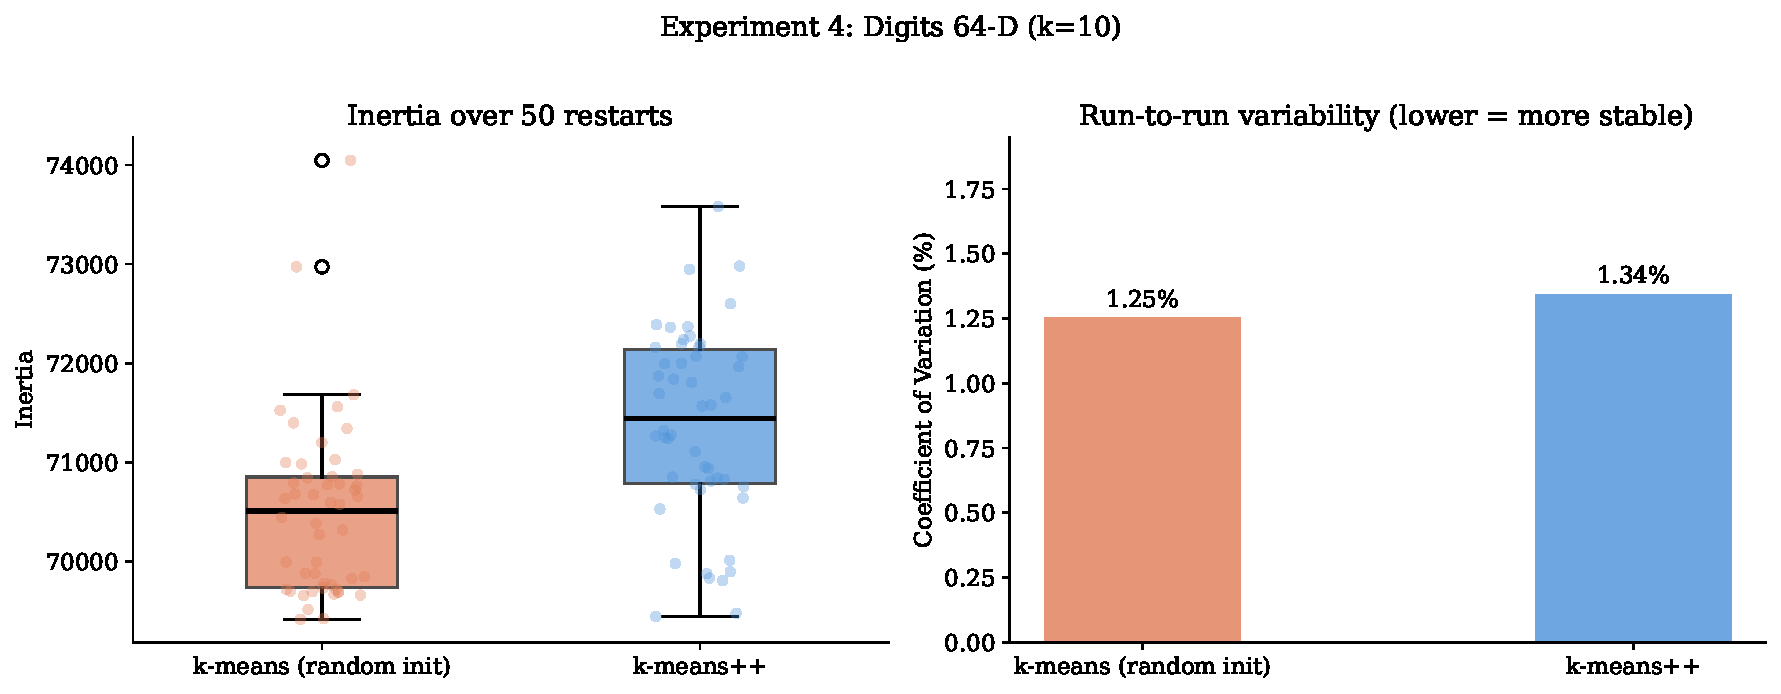
\includegraphics[width=\linewidth]{figures/exp4_digits.pdf}
  \caption{Digits 64-D: nearly identical, very tight inertia distributions (CV
           $\approx1.3\%$ for both), suggesting a much smoother objective landscape than
           in Experiment 1.}
  \label{fig:exp4}
\end{figure}

The result \textbf{inverts}. $k$-means++ is marginally \emph{worse}: inertia $+1.3\%$,
ARI 0.464 vs \textbf{0.512}, NMI 0.618 vs \textbf{0.656}. We did not isolate a single
cause experimentally, but several mechanisms are consistent with this behaviour:

\begin{enumerate}[nosep,leftmargin=*]
  \item \textbf{Distance concentration.} In 64 dimensions pairwise distances tend to
        concentrate ($\max/\min\to1$), which would flatten the $D^2$ distribution and
        make $k$-means++ sampling closer to uniform, weakening the seeding signal. This
        is a plausible contributing factor rather than one we measure directly here.
  \item \textbf{Smoother landscape.} CV $\approx1.3\%$ for \emph{both} methods —
        roughly 50$\times$ lower than Experiment 1. This low restart-to-restart spread
        suggests a substantially less multimodal landscape, in which the starting point
        matters little for final inertia; we infer this from the variability, not from a
        direct characterization of the basins.
  \item \textbf{Greedy spreading on outliers.} $k$-means++ maximizes spread, which may
        anchor seeds on atypical digit images. Such outlier seeds could attract few
        points, producing unbalanced clusters that score worse on ARI/NMI.
  \item \textbf{Standardization.} We standardize all 64 features; several are
        near-constant edge pixels whose variance is dominated by noise. Standardization
        inflates the influence of these low-signal dimensions on the Euclidean distance,
        which may itself disadvantage the spread-maximizing $D^2$ seeding. Unlike the
        first three, this is directly testable by re-running without standardization
        (noted under Limitations).
\end{enumerate}

\textbf{Methodological lesson.} Inertia alone would suggest equivalence (both
$\approx70{,}000$, CV $\approx1.3\%$). Only external metrics reveal the reversal and
its direction. A study relying only on the internal objective would miss this entirely.

\subsection{External validation across datasets}

\begin{figure}[H]
  \centering
  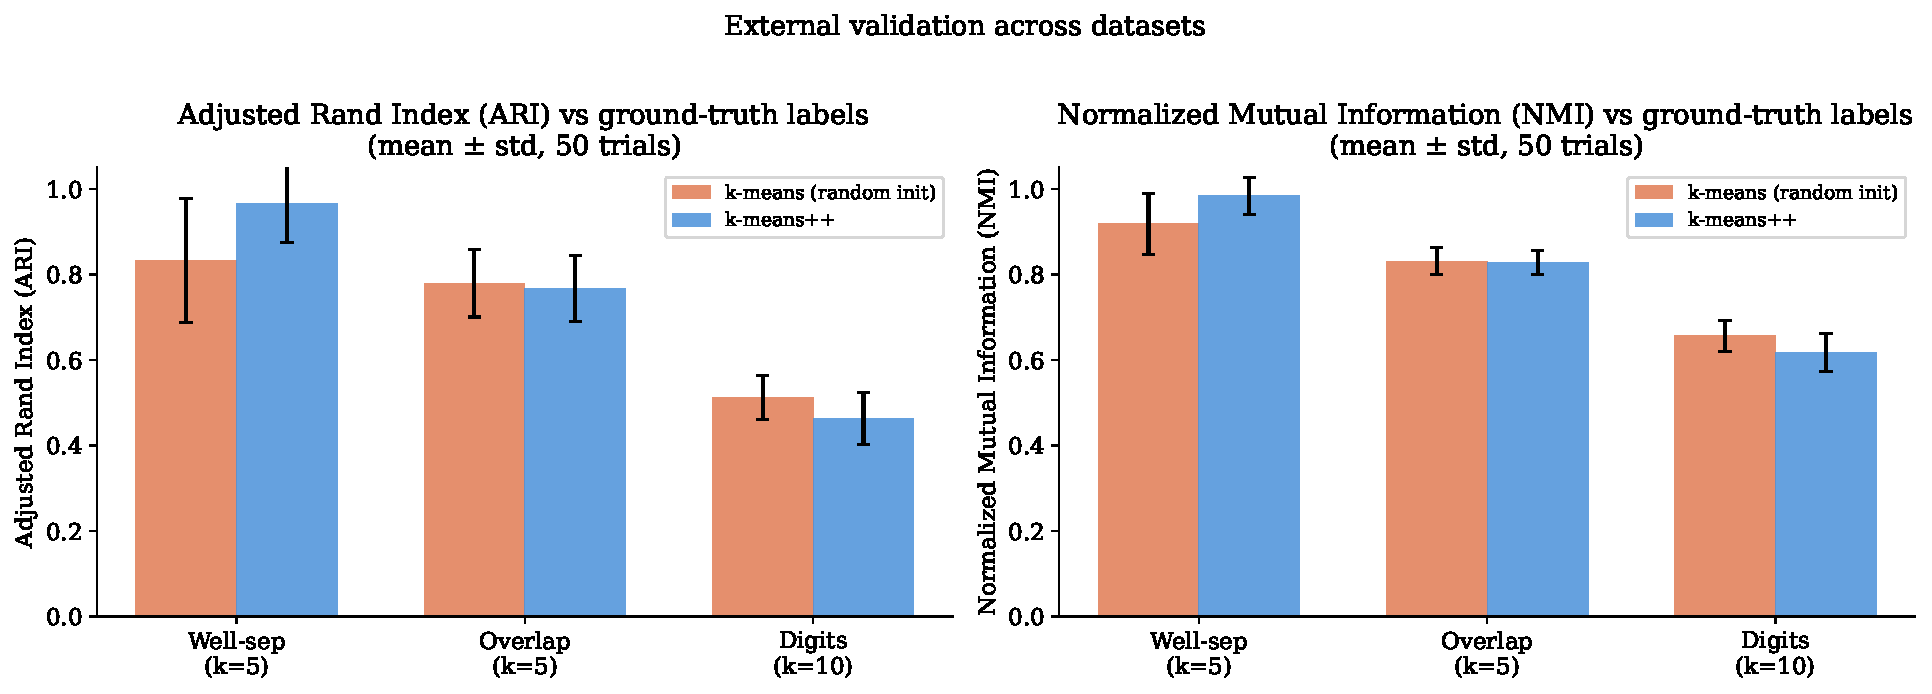
\includegraphics[width=\linewidth]{figures/exp_external.pdf}
  \caption{ARI and NMI across all three labelled datasets (mean $\pm$ 1 std, 50 restarts).
           $k$-means++ leads only on well-separated data; ties on overlapping;
           trails on Digits.}
  \label{fig:external}
\end{figure}

Figure~\ref{fig:external} places all three regimes side by side. The pattern is
unambiguous: $k$-means++ improves ARI by $+0.13$ on well-separated data, matches random
on overlapping data, and trails by $-0.05$ on Digits. The error bars confirm that random
init is most variable on well-separated data (wide) and barely variable on Digits (narrow),
consistent with the landscape-structure story across all experiments.

% ════════════════════════════════════════════════════════════════════════════
\section{Summary and Discussion}
% ════════════════════════════════════════════════════════════════════════════

\begin{table}[H]
\centering\small
\caption{Full cross-dataset summary (50 restarts, \texttt{random\_state=42}).
  $\Delta J\%$: percentage reduction in mean $J$ by $k$-means++; positive = better.}
\label{tab:summary}
\setlength{\tabcolsep}{4.5pt}
\begin{tabular}{lrrrrrrrrrr}
\toprule
\textbf{Dataset} & $\bar{J}_r$ & $\bar{J}_{++}$ & $\Delta J$\%
  & CV$_r$ & CV$_{++}$ & ARI$_r$ & ARI$_{++}$ & NMI$_r$ & NMI$_{++}$
  & it$_r$/it$_{++}$ \\
\midrule
Well-sep (2D, $k$=5) & 1109 & 439
  & \textbf{+60.4} & 80.2 & 75.5 & 0.833 & \textbf{0.966}
  & 0.919 & \textbf{0.984} & 5.6 / \textbf{3.1} \\
Overlap (2D, $k$=5) & 2915 & 2931
  & $-0.5$ & 14.5 & \textbf{9.3} & 0.780 & 0.768
  & 0.832 & 0.828 & 11.3 / \textbf{9.4} \\
Digits (64D, $k$=10) & 70493 & 71381
  & $-1.3$ & 1.3 & 1.3 & \textbf{0.512} & 0.464
  & \textbf{0.656} & 0.618 & 25.6 / 25.1 \\
\bottomrule
\end{tabular}
\end{table}

The experiments reveal a nuanced picture, consistent with both the theoretical
guarantees of $k$-means++ and the conditions under which they stop being useful.

\textbf{Finding 1 — Strong structure: $k$-means++ outperforms clearly.}
A 60.4\% inertia reduction, ARI from 0.833 to 0.966, NMI from 0.919 to 0.984, half the
iterations, and 88\% near-optimal rate vs 42\% for random init. The scatter plots
illustrate the mechanism: $D^2$ seeding prevents the pathological two-seeds-in-one-cluster
initialization that Lloyd often cannot recover from.

\textbf{Finding 2 — Weak structure: stability and speed, not quality.}
Both methods reach the same partition quality (ARI $\approx0.77$). $k$-means++ still
reduces CV by 36\% and cuts iterations from 11.3 to 9.4, which matters in any
single-run or time-constrained setting.

\textbf{Finding 3 — High dimensions: the advantage reverses.}
On 64-D Digits, $k$-means++ is marginally worse on inertia, ARI, and NMI. Several factors
are consistent with this: distance concentration likely weakens the $D^2$ signal, the
landscape appears far less multimodal (very low CV), greedy spreading may misplace seeds
on outlier images, and feature standardization may itself disadvantage spread-based seeding.
This negative result is only visible through external metrics.

\textbf{Finding 4 — Growing advantage with $k$.}
The inertia ratio grows monotonically from 1.01 at $k=2$ to 1.82 at $k=15$, qualitatively
consistent with the O$(\log k)$ guarantee: as $k$ grows, random init has more chances to
mis-seed. The inter-method ratio is a distinct quantity from the bound's $\ln k$ factor and
we make no claim that the two match numerically.

\textbf{Visualization choices.} Box-and-strip plots expose the full inertia distribution
(not just mean $\pm$ std), making bimodal outcomes visible. The scatter triptych (worst/typical/best)
illustrates the failure mechanism directly. The convergence curve uses the median run to
avoid cherry-picking; bar charts include error bars for variability.

% ════════════════════════════════════════════════════════════════════════════
\section{Conclusions}
% ════════════════════════════════════════════════════════════════════════════

$k$-means++ is a strong default whose benefit is \emph{conditional} on strong,
low-dimensional structure and large $k$, broadly in line with the O$(\log k)$ theory.
The key lesson is that initialization studies must pair inertia with external
label-based metrics (ARI, NMI) and a stability measure; inertia alone conceals
both the high-dimensional reversal and the overlapping null result.

\textbf{Limitations.}
(i)~Synthetic datasets are isotropic equal-sized Gaussians; real clusters are often non-spherical.
(ii)~The Digits reversal is reported from standardized features; re-running on raw (unstandardized)
features and with PCA would test whether standardization or distance concentration drives the effect,
and is the most direct follow-up to the Section~5.4 discussion.
(iii)~Convergence tolerance $10^{-4}$ may not fully converge on Digits; a tighter threshold
would cost more iterations.
(iv)~The Digits ARI gap (0.512 vs 0.464) is small relative to its run-to-run spread; we report
it as a difference in mean external metrics rather than a statistically established effect.

\textbf{Future directions.}
Apply PCA before Digits clustering; compare with $k$-means$\|$ [4]
(parallel $O(\log n)$-round seeding); extend to mini-batch $k$-means and non-Euclidean
settings.


\enlargethispage{4\baselineskip}
% ── References ──────────────────────────────────────────────────────────────
\vspace{3pt}
{\large\bfseries References}\\[-4pt]
\rule{\linewidth}{0.4pt}\vspace{0pt}
{\footnotesize
\begin{description}[leftmargin=1.8em, labelindent=0pt, itemsep=1pt, parsep=0pt, topsep=0pt]
  \item[[1]] Arthur, D.\ \& Vassilvitskii, S.\ (2007). $k$-means++: The advantages of careful seeding. In \textit{Proc.\ ACM-SIAM SODA}, pp.\ 1027--1035.
  \item[[2]] Lloyd, S.\ P.\ (1982). Least squares quantization in PCM. \textit{IEEE Trans.\ Inf.\ Theory}, 28(2):129--137.
  \item[[3]] Hubert, L.\ \& Arabie, P.\ (1985). Comparing partitions. \textit{J.\ Classification}, 2:193--218.
  \item[[4]] Bahmani, B.\ et al.\ (2012). Scalable $k$-means++. \textit{Proc.\ VLDB Endowment}, 5:622--633.
\end{description}}
\end{document}
% already at end — patch bibliography font size before \end{document}
